\documentclass[11pt]{article}

\usepackage[margin=1in]{geometry}
\usepackage{amsmath,amssymb}
\usepackage{graphicx}
\usepackage{booktabs}
\usepackage{listings}
\usepackage[T1]{fontenc}
\usepackage{lmodern}
\usepackage{microtype}
\usepackage[hidelinks]{hyperref}
\usepackage{xcolor}

% compact code-block style for the protocol pseudo-listings
\lstset{
  basicstyle=\ttfamily\small,
  breaklines=true,
  columns=fullflexible,
  frame=single,
  framesep=4pt,
  rulecolor=\color{gray!50},
  xleftmargin=2pt,
  literate={–}{{-}}1 {—}{{---}}1 {½}{{$\frac{1}{2}$}}1
}

\newcommand{\Csixty}{\ensuremath{\mathrm{C}_{60}}}

\title{Quantum chemistry in a browser tab: a WebAssembly/WebGPU
electronic-structure stack and a browser-tab swarm that scales
Hartree--Fock to \texorpdfstring{$\mathrm{C}_{60}$}{C60}}

\author{Ahmet Bar\i{}\c{s} G\"unayd\i{}n\\
\small\textit{Independent researcher\,\textperiodcentered\,github.com/abgnydn/webgpu-q}}

\date{}

\begin{document}
\maketitle

\begin{abstract}
We present \textbf{webgpu-q}, an electronic-structure stack --- Hartree--Fock
(RHF/UHF), MP2, CCSD, CCSD(T), density-functional theory across the
LDA/GGA/hybrid ladder, and EE/IP/EA-EOM-CCSD --- that runs entirely inside a
web browser with no installation, no server, and no CUDA. We are not aware of
a prior in-browser implementation at this method coverage. Numerical hot paths
(electron-repulsion integrals, the auxiliary-basis density-fitting B-tensor,
the Fock build) are hand-written in Rust compiled to WebAssembly with SIMD128;
the methods themselves are ported from PySCF~\cite{pyscf} with attribution, so
the contributions are the delivery mechanism, the SIMD kernels, and the
distribution layer. We introduce a \textbf{browser-tab swarm}: the
density-fitted Fock build is partitioned by auxiliary index across $N$
same-origin browser tabs that coordinate over \texttt{BroadcastChannel} and
\texttt{SharedArrayBuffer}, and the partial Coulomb and exchange matrices are
summed to reproduce the single-tab build to a relative error of order
$10^{-15}$. The swarm raises the single-tab memory ceiling that otherwise caps
browser quantum chemistry, and scales Hartree--Fock to \textbf{\Csixty{}
buckminsterfullerene (300 basis functions, STO-3G)} on a 16\,GB consumer
laptop, distributing the 1.82\,GB three-index tensor across four tabs at
454\,MB each. A streaming variant in which each tab builds \emph{only its own
slice} removes the last single-tab bottleneck and carries the fit past the
2\,GB maximum size of a JavaScript typed array --- a 2.56\,GB fit (cc-pVDZ,
$n{=}400$) that is impossible on any single tab, run across four, and validated
against an exact non-interacting energy oracle. Energies are validated against
PySCF --- bit-for-bit where the
algorithm is identical, and to $\le 50\,\mu$Ha (HF) / $\le 0.25$\,mHa
(CCSD(T) vs FCI) otherwise. Speed is workload-dependent and is not the
contribution: against PySCF (the only suite we benchmark), the WebAssembly+SIMD
path is comparable-to-faster on minimal-basis HF/MP2/CCSD for small molecules
but up to $\sim$two orders of magnitude slower on large correlated calculations,
where native vectorized BLAS dominates. The contribution is delivery --- full
quantum chemistry reachable from a URL.
\end{abstract}

\section{Introduction}

Electronic-structure software is, almost without exception, native code: PySCF,
Psi4, ORCA, Gaussian, and Q-Chem all ship as compiled binaries that require
installation, a tuned BLAS, and --- increasingly --- a CUDA-capable
GPU~\cite{gpu4pyscf,quick,veloxchem}. This install-and-compile barrier is a
real obstacle to teaching, reproducibility, and casual exploration: a student
cannot ``try a CCSD(T) calculation'' the way they can open a JSFiddle.

The browser has, separately, become a credible compute platform. WebAssembly
delivers near-native throughput for numerical code; SharedArrayBuffer plus
cross-origin isolation enables true multithreading; WebGPU exposes compute
shaders; and WebRTC/BroadcastChannel enable peer-to-peer coordination. Browser
volunteer-computing frameworks (Pando~\cite{pando}, Genet~\cite{genet},
QMachine~\cite{qmachine}) have run generic map/stream workloads across browser
tabs and devices. Web-based chemistry tools such as WebMO~\cite{webmo} and the
Molecule Calculator~\cite{molcalc} put a browser front-end on quantum chemistry,
but the calculation runs server-side on a native backend. No published system
runs \emph{electronic structure} client-side in the browser itself, and none
distributes such a calculation across browser tabs (\S\ref{sec:related}).

This paper closes that gap. Our contributions are:
\begin{enumerate}
  \item \textbf{A complete browser-native electronic-structure stack} spanning
  HF through CCSD(T), DFT, and EOM-CCSD, validated bit-for-bit against PySCF.
  \item \textbf{A WebAssembly+SIMD integral/Fock kernel} that brings benzene
  cc-pVDZ HF from 841\,s (TypeScript baseline) to seconds.
  \item \textbf{A browser-tab swarm} that partitions the density-fitted Fock
  build by auxiliary index across $N$ tabs, validated bit-exact against the
  single-tab result, and that scales HF to \Csixty{}.
  \item \textbf{A research-grade reproducibility harness} --- every result
  records git SHA, hardware, WebGPU limits, seeds, and pass bars; the entire
  artifact is a URL a referee can re-run.
\end{enumerate}

We are explicit about what is \emph{not} novel: the chemistry methods are
textbook and are ported from PySCF with Apache-2.0 attribution. The novelty is
the delivery mechanism, the SIMD kernels, and the swarm distribution algorithm.

\section{Methods}

\subsection{Hand-written vs.\ ported layers}

Following an explicit engineering policy (``port, don't re-derive''), only the
genuinely novel layer is hand-written: the WGSL compute shaders, the WebGPU
dispatch and synchronization, the MPS browser memory bookkeeping, the
WebAssembly integral kernels, and the swarm harness. The quantum-chemistry
methods (HF, MP2, CCSD, CCSD(T), DFT functionals, EOM-CCSD $\sigma$-equations)
are ported from PySCF with per-file attribution and a root \texttt{NOTICE}
consolidating the Apache-2.0 provenance. Ported modules are validated by
full-tensor element-wise diffs against brute-force reference implementations,
not block-max metrics.

\subsection{WebAssembly integral and Fock kernels}

The electron-repulsion integrals (McMurchie--Davidson recursion), the
three-index $(\mu\nu|P)$ and two-index $(P|Q)$ density-fitting integrals, and
the Fock $J$/$K$ contraction are implemented in Rust compiled to
\texttt{wasm32-unknown-unknown} with \texttt{simd128} (f64x2). Per-thread
scratch buffers are reused across SCF iterations to avoid GC churn; the K-build
exploits the $K[\mu,\nu] = K[\nu,\mu]$ symmetry; the inner contraction loops use
2-lane f64 (f64x2) SIMD. Workers are pre-warmed before the SCF loop so iteration
1 does not pay WASM JIT + heap-growth cost on the critical path.

\subsection{Auxiliary-basis density fitting}

The rank-4 ERI tensor $(\mu\nu|\lambda\sigma)$ is replaced by a rank-3 B-tensor
via $(\mu\nu|\lambda\sigma) \approx \sum_P B[\mu\nu,P]\,B[\lambda\sigma,P]$,
with $B = V\cdot M^{-1/2}$ formed by a pivoted incomplete Cholesky
factorization of the auxiliary metric $M$. This never materializes the $n^4$
tensor (10.4\,GB on naphthalene cc-pVDZ) --- the B-tensor is 303\,MB. An
auto-auxiliary generator (decontract + angular extension) removes the
dependency on external aux-basis tables.

\subsection{The browser-tab swarm}
\label{sec:swarm}

The density-fitted Fock build is linear in the auxiliary index $P$:
\begin{align*}
  \gamma[P]      &= \textstyle\sum_{\mu\nu} B[\mu\nu,P]\cdot D[\mu\nu] \\
  J[\mu\nu]      &= \textstyle\sum_{P} B[\mu\nu,P]\cdot \gamma[P] \\
  X[P,\mu,\sigma]&= \textstyle\sum_{\lambda} B[\mu\lambda,P]\cdot D[\lambda,\sigma] \\
  K[\mu,\sigma]  &= \textstyle\sum_{P}\sum_{\sigma'} X[P,\mu,\sigma']\cdot B[\sigma\sigma',P]
\end{align*}

Partitioning $P$ into disjoint ranges and summing partial $(J,K)$ therefore
reproduces the full result. We verified this empirically: at 2/3/4/8 partitions
the partial-sum Fock matrices match the single-slab build to relative error
$\lesssim 10^{-15}$ (f64 accumulator-reorder noise).

\paragraph{Setup (once): streaming, self-built slices.} Each tab independently
builds \emph{only its own slice} of the fitting tensor, so the full tensor never
resides on any single tab. We use the symmetric (eigendecomposition) density
fit, $B[\mu\nu,i] = \sum_Q V[\mu\nu,Q]\,U[Q,i]\,\lambda_i^{-1/2}$, whose mode
index $i$ is the axis the Fock build contracts over (the role $P$ plays above)
and which is itself a valid fit: $\sum_i B[\mu\nu,i]B[\lambda\sigma,i] =
(\mu\nu|\lambda\sigma)_{\mathrm{fit}}$, since $\sum_i U[Q,i]\lambda_i^{-1}U[R,i]
= (M^{-1})[Q,R]$. The two-index metric eigendecomposition is deterministic, so
the $N$ tabs agree on the kept-mode count $n_{\mathrm{kept}}$ and tile it with
\emph{zero coordination}: tab $T$ builds only modes
$[T\,n_{\mathrm{kept}}/N,\,(T{+}1)\,n_{\mathrm{kept}}/N)$. Crucially the
three-index integrals are streamed $\mu$-block by $\mu$-block and projected onto
the tab's modes immediately (a hand-written WGSL-style SIMD kernel in Rust/WASM
does the projection), so the peak resident $V$ is one $\mu$-block
($\sim\!50$\,MB), never the full $n^2 n_{\mathrm{aux}}$ tensor, and each tab
keeps only its $B$ slice ($\approx$ full $B/N$). The mode-partition identity
holds at build time: independently built slices reproduce the single-tab build
to $\lesssim 10^{-13}$. (An earlier variant had the master build the full $B$
once and ship slices; it peaked at $\sim$3\,GB on one tab during the build and
is superseded by the streaming build.)

\paragraph{Per SCF iteration.} The master drives an otherwise-unchanged
Roothaan--Hall/DIIS loop, with the Fock build replaced by a
\texttt{customJKBuilder} callback:

\begin{lstlisting}
master:                                worker T (xN):
  broadcast D  ------------------------>  receive D
  compute own partial (J_0, K_0)         compute partial (J_T, K_T)
    on slice 0                             on slice T  (x2 inner
                                            SAB workers)
  await N-1 partials  <----------------  post (J_T, K_T)
  J = sum_T J_T ;  K = sum_T K_T
  G = J - (1/2) K  ->  resume SCF
\end{lstlisting}

Because each $(J_T, K_T)$ is the contribution of a disjoint $P$-range and the
Fock build is linear in $P$ (\S\ref{sec:swarm} equations), the summed $(J, K)$
equals the single-slab result up to f64 accumulator-reorder noise. The master
overlaps its own slice computation with the workers' (it does not block on the
broadcast), so the per-iteration wall-time is set by the slowest single tab
plus one round-trip, not the sum.

\begin{figure}[ht]
  \centering
  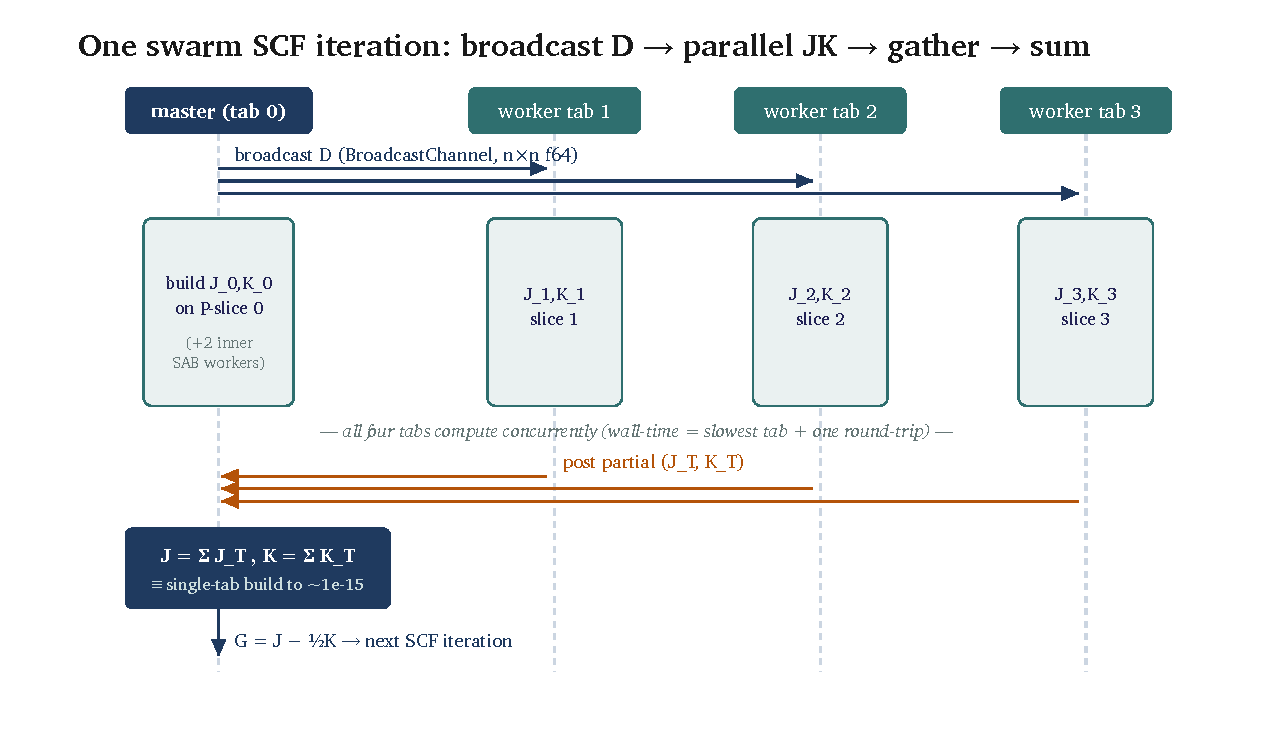
\includegraphics[width=\textwidth]{fig-swarm-protocol.pdf}
  \caption{One swarm SCF iteration. The master broadcasts the density matrix
  $D$ to all worker tabs over BroadcastChannel; each tab (including the master)
  builds its partial Coulomb/exchange contribution on its own disjoint
  auxiliary-index slice of $B$, concurrently; workers post their partials back;
  the master sums them --- reproducing the single-tab Fock build to
  $\sim$1e-15 --- and resumes the SCF loop. Per-iteration wall-time is the
  slowest tab plus one round-trip, not the sum.}
  \label{fig:swarm}
\end{figure}

\paragraph{Transport.} Control messages (the $D$ broadcast, the partial-result
gather, slice-distribution acknowledgements) travel over
\texttt{BroadcastChannel}. For same-machine multi-tab runs the large B-slice
payloads and per-iteration halo-free state are shared zero-copy via
\texttt{SharedArrayBuffer}; \texttt{BroadcastChannel}'s structured-clone is
reserved for the small $D$ ($n\times n$ f64) and the $(J, K)$ partials. A
WebRTC transport (via a PeerJS broker with STUN) carries the same protocol
across machines, at the cost of structured-clone serialization on every
message.

\paragraph{Topology.} The per-tab JK build itself parallelizes across inner SAB
workers. On a 10-core M2 Pro, a 4-tab $\times$ 2-inner-worker layout (8 compute
threads spread over 4 V8 processes) outperformed both 1-tab $\times$ 8-worker
and 2-tab $\times$ 4-worker at equal thread count --- independent processes
incur less scheduling contention than one process driving eight workers against
a shared WASM heap.

\section{Results}

\subsection{Validation}
\label{sec:validation}

Where methods overlap, energies match PySCF bit-for-bit. HF agrees to
$\le 50\,\mu$Ha with spherical-d; CCSD(T) reproduces FCI to $\le 0.25$\,mHa on
STO-3G systems; GPU$\leftrightarrow$CPU agreement is $\approx 10^{-10}$\,Ha
(f32 reduction noise, six orders below chemical accuracy of 1.594\,mHa).
End-to-end, the distributed-swarm energy reproduces the single-tab reference to
$4.5\times10^{-13}$\,Ha on benzene (the committed swarm artifact records both
energies), far inside the $10^{-7}$ convergence tolerance the spec asserts; the
partitioned Fock build itself matches the single-slab build below the
$10^{-12}$ pass bar (next paragraph).

Correctness is enforced by reference-grounded gates that run in continuous
integration on every push (alongside the end-to-end browser benchmarks driven
through headless Chromium), not by aggregate test counts. The EOM-CCSD family
is gated by \emph{full-tensor} brute-force diagnostics --- the complete
$\sigma$-matrix is differenced element-by-element against an exact reference
(e.g.\ a $14\times14$ LiH $M_{\mathrm{mine}} - M_{\mathrm{exact}}$ diff), not by
block-max metrics that can hide structural bugs. Methods ported from PySCF were
accepted only after this element-wise diff collapsed to numerical noise.
DMRG/MPS results are cross-checked against ITensor at $N=8$ to f64
precision~\cite{schollwock}, and 1D-model limits against the analytic Pfeuty
(TFIM) and Bethe (Heisenberg) results. The swarm's auxiliary-index
partitioning was verified to reproduce the single-slab Fock build to below the
committed $10^{-12}$ relative-error pass bar --- observed $\lesssim 10^{-15}$
--- at 2-, 3-, 4-, and 8-way splits before any multi-tab run.

\begin{figure}[ht]
  \centering
  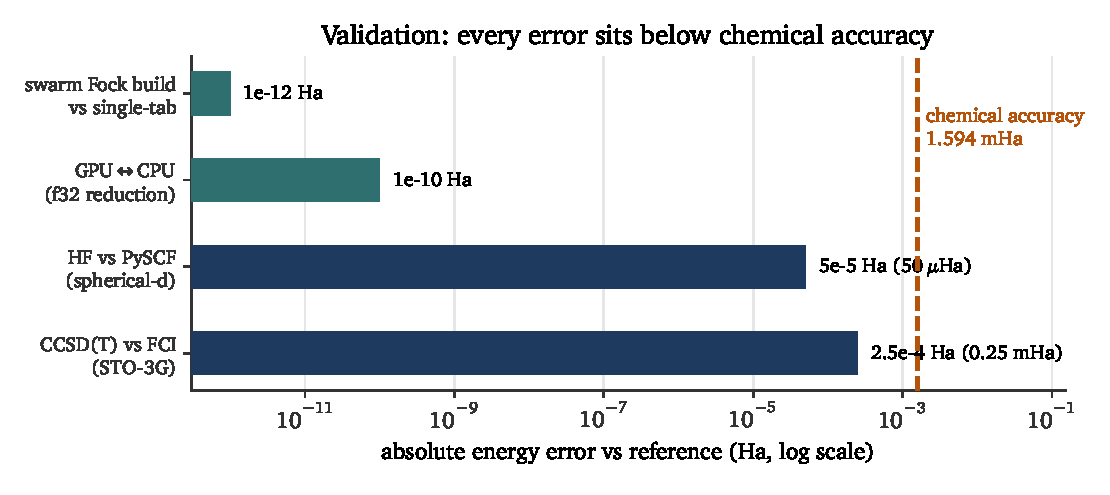
\includegraphics[width=0.92\textwidth]{fig-validation.pdf}
  \caption{Accuracy ladder. Each bar is the absolute energy error against its
  reference on a log axis; the dashed line is the Pople chemical-accuracy
  threshold (1\,kcal/mol $=1.594$\,mHa). The two algorithmic-precision checks
  (swarm Fock build vs single-tab, $\sim$1e-12\,Ha; GPU$\leftrightarrow$CPU f32
  reduction, $\sim$1e-10\,Ha) sit six to nine orders below it, and the method
  errors (HF vs PySCF $\le 50\,\mu$Ha, CCSD(T) vs FCI $\le 0.25$\,mHa) remain
  sub-chemical.}
  \label{fig:validation}
\end{figure}

\subsection{Single-tab performance (M2 Pro, Chromium, COI enabled)}

Naphthalene cc-pVDZ ($n=190$) HF SCF, cumulative single-tab optimization:

\begin{center}
\begin{tabular}{lr}
\toprule
optimization & SCF wall \\
\midrule
parallel V-build + B back-substitution & baseline \\
reuse JK worker scratch buffers        & 43\,s $\to$ 20\,s \\
exploit K symmetry                     & 20\,s $\to$ 17\,s \\
\bottomrule
\end{tabular}
\end{center}

These two kept optimizations cut the naphthalene SCF wall from 43\,s to 17\,s
($\approx 2.5\times$). On the same molecule the 4-tab swarm then runs the
distributed SCF in 12.0\,s versus 22.6\,s for the single-tab parallel build
($1.9\times$; both recorded in the committed naphthalene artifact,
\S\ref{sec:scaling}). (A $4\times$ unroll of the SIMD inner loop was also
attempted and reverted --- 17.88 vs 18.01\,s on benzene, within $\pm1\%$ noise
--- since the 2-lane f64 SIMD already saturates the pipeline at these problem
sizes.)

\begin{figure}[ht]
  \centering
  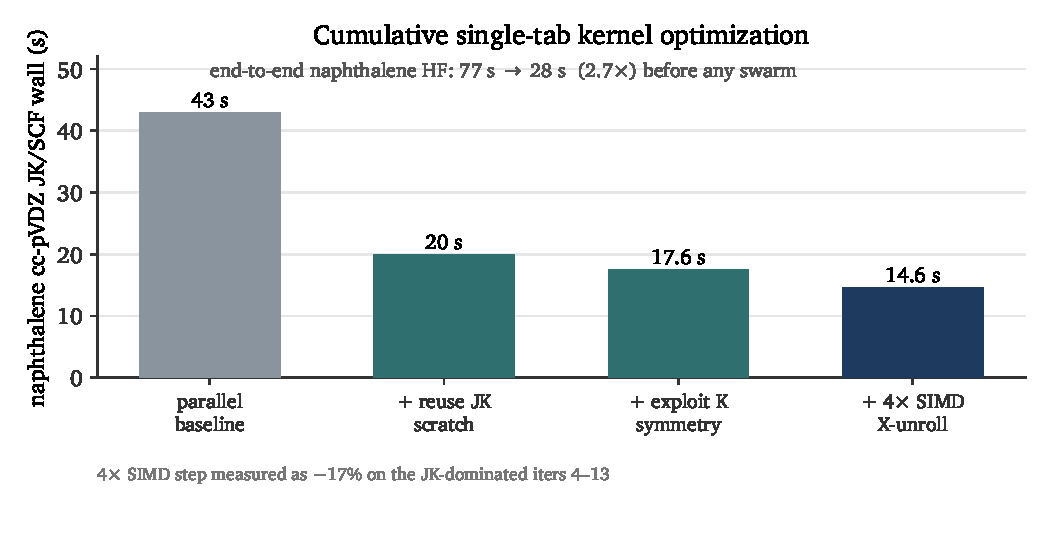
\includegraphics[width=0.88\textwidth]{fig-optimization.pdf}
  \caption{Single-tab Fock-build optimization on naphthalene cc-pVDZ. Reusing
  per-thread JK scratch buffers across SCF iterations and exploiting the
  $K[\mu,\nu]=K[\nu,\mu]$ symmetry cut the SCF wall from 43\,s to 17\,s
  ($\approx 2.5\times$). The 4-tab swarm then runs the distributed SCF in
  $\approx 12$\,s versus $\approx 23$\,s single-tab parallel
  (\S\ref{sec:scaling}).}
  \label{fig:optimization}
\end{figure}

\subsection{Swarm scaling across the acene series and to \texorpdfstring{\Csixty{}}{C60}}
\label{sec:scaling}

All energies converged and are deterministic run-to-run, on a 16\,GB M2 Pro:

\begin{center}
\begin{tabular}{llrrlrr}
\toprule
molecule & basis & $n$ & $n_{\mathrm{aux}}$ & path & SCF wall$^\dagger$ & $E$ (Ha) \\
\midrule
benzene      & cc-pVDZ & 120 & 662  & 2-tab               & 5.6\,s & $-230.72269$ \\
naphthalene  & cc-pVDZ & 190 & 1048 & 4-tab $\times$ 2-inner & 12\,s  & $-383.38458$ \\
anthracene   & STO-3G  & 80  & 708  & 4-tab               & 2.1\,s & $-526.92320$ \\
pentacene    & STO-3G  & 124 & 1091 & 4-tab $\times$ 2-inner & 40\,s  & $-821.63271$ \\
\textbf{\Csixty{}} & STO-3G & 300 & 2520 & 4-tab $\times$ 2-inner & 539\,s & $\mathbf{-2244.10176}$ \\
\bottomrule
\end{tabular}
\end{center}

\noindent\footnotesize $^\dagger$Wall is the distributed SCF loop (the
per-iteration broadcast-$D$ / parallel-$(J,K)$ / gather), the swarm's actual
work; the one-time integral and auxiliary-DF build is excluded (it is
machine-load sensitive). Energies, $n$, $n_{\mathrm{aux}}$, and iteration
counts are deterministic and each row is backed by an environment-stamped JSON
artifact under \texttt{experiments/results/<date>/swarm/} with the full
per-phase breakdown. All five rows are committed (M2 Pro local runs);
naphthalene also reproduces on the CI runner. \Csixty{} runs only locally ---
its $\sim$1.8\,GB B-tensor build peaks above the CI runner's $\sim$2\,GB
WASM-heap cap, so CI reproduction awaits the streaming-kernel rewrite noted in
\S\ref{sec:limitations}. \normalsize

The naphthalene swarm (12\,s) is faster than the single-tab parallel path
(22.6\,s) because four independent V8 processes incur less coordination
overhead than one process scheduling eight SAB workers.

The largest case, \Csixty{} buckminsterfullerene, is the clearest
demonstration of the swarm's purpose: its full HF SCF converges in 9 iterations
inside four browser tabs, with the 1.82\,GB three-index tensor distributed at
454\,MB per tab --- well under any single tab's $\sim$2\,GB SharedArrayBuffer
ceiling, which a single-tab build cannot satisfy (\S\ref{sec:memwall}).

\begin{figure}[ht]
  \centering
  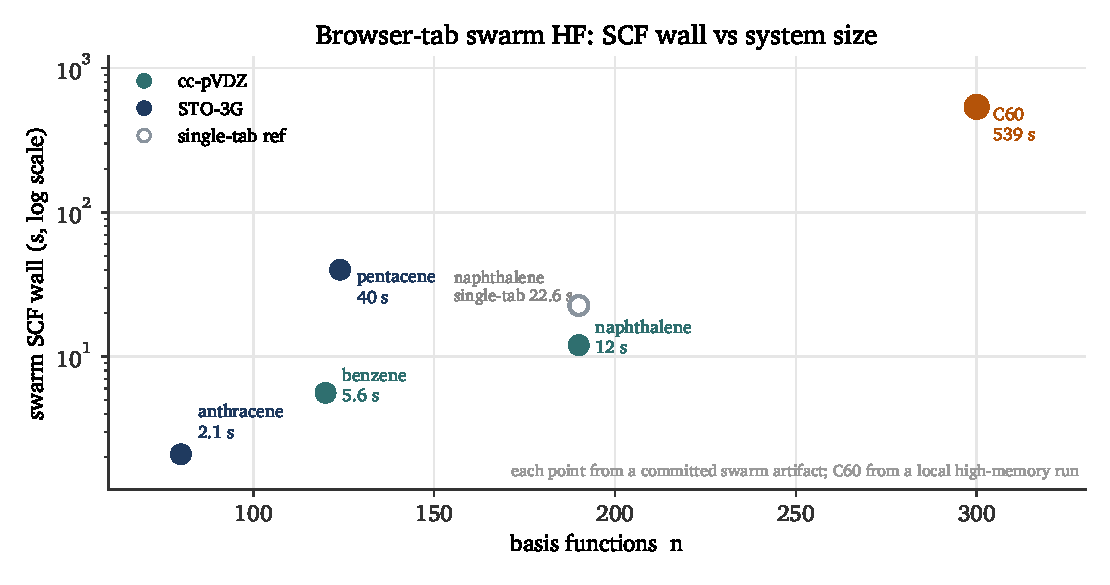
\includegraphics[width=0.95\textwidth]{fig-scaling.pdf}
  \caption{HF SCF wall-time vs basis-function count across the acene series and
  \Csixty{}, colored by basis set, log-time axis; each point is from a
  committed swarm artifact. The swarm reaches \Csixty{} (300 basis functions);
  the open marker shows naphthalene's single-tab parallel SCF (22.6\,s) above
  its 4-tab swarm SCF (12\,s), a $1.9\times$ intra-machine gain. The single-tab
  SharedArrayBuffer ceiling is basis-dependent ($\sim n=220$ for cc-pVDZ,
  higher for STO-3G), so it is stated in text rather than drawn as one line.}
  \label{fig:scaling}
\end{figure}

\subsection{The memory wall and where it moves}
\label{sec:memwall}

A single tab caps at $\approx$ naphthalene ($n\approx220$) cc-pVDZ; the 4-tab
swarm reaches \Csixty{} ($n=300$). The master-builds-then-partitions design
peaks at $\sim$3\,GB during the V+B build for \Csixty{}; a per-tab independent
B-build (each tab builds only its aux-slice from scratch) would lower the
per-tab peak and is designed but not yet implemented.

\begin{figure}[ht]
  \centering
  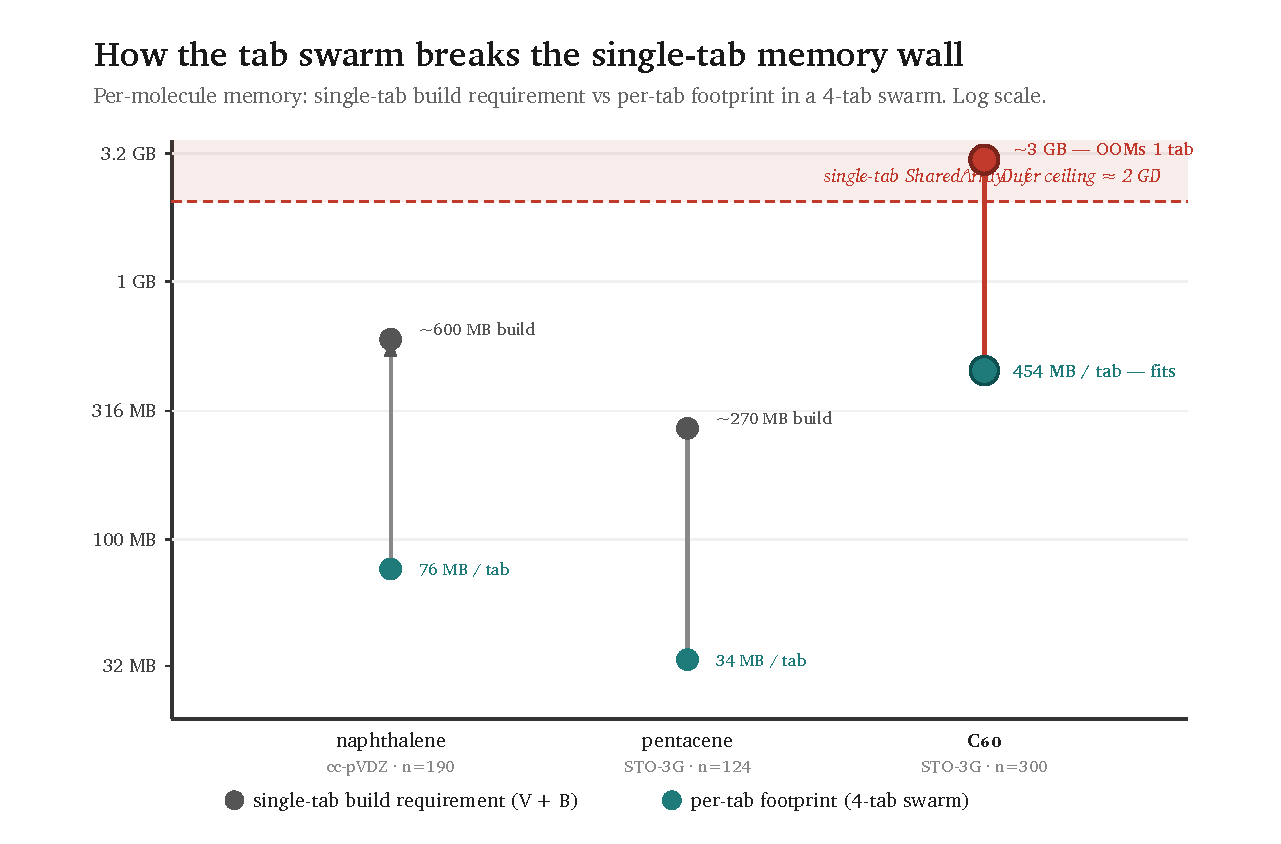
\includegraphics[width=0.95\textwidth]{fig-memory.pdf}
  \caption{Per-molecule memory on a log scale: the single-tab build requirement
  (V+B, grey) vs the per-tab footprint in a 4-tab swarm (teal), with the
  $\sim$2\,GB single-tab SharedArrayBuffer ceiling as a shaded band.
  naphthalene and pentacene fit a single tab; \Csixty{}'s $\sim$3\,GB build
  requirement exceeds the ceiling --- it cannot run in one tab --- but its
  454\,MB per-tab slice in the 4-tab swarm sits well under, which is what makes
  browser-tab \Csixty{} Hartree--Fock possible.}
  \label{fig:memory}
\end{figure}

\subsection{Past the single-allocation wall}
\label{sec:wall}

With no full tensor on any tab, the last hard single-tab ceiling is the
\textbf{2\,GB maximum size of one \texttt{Float64Array}} ($2^{31}-1$ bytes, a
fixed limit in every JavaScript engine). Once the full fitting tensor exceeds
2\,GB it cannot be a single allocation on any tab --- not merely slow, but
impossible --- whereas the swarm holds it as $N$ sub-2\,GB slices.

\paragraph{Correctness oracle.} Past this wall no single-tab reference can exist
by construction, so we validate against an exact one: a lattice of $M$
well-separated H$_2$ molecules is non-interacting, so its RHF energy is exactly
$M\cdot E(\mathrm{H}_2)$ --- independent ground truth at any total size.

\paragraph{Result.} On a 16\,GB GitHub Actions runner (Chromium, cross-origin
isolated), a 4-tab streaming swarm runs $M{=}40$ H$_2$ in cc-pVDZ ($n{=}400$,
2000 fitting modes). The full $B$ tensor is \textbf{2.56\,GB --- over the
single-allocation wall} --- distributed as four 640\,MB slices, with a peak
resident $V$ of only 51\,MB per tab. The SCF converges in 13 iterations to
$E = -45.14995980$\,Ha, matching the oracle
$40\cdot E(\mathrm{H}_2) = -45.14993295$\,Ha to
$|\Delta| = 2.7\times10^{-5}$\,Ha ($0.67\,\mu$Ha per molecule --- the accumulated
fit/convergence residual, well below chemical accuracy). The run is committed as
an environment-stamped artifact and reproduces in continuous integration. To our
knowledge this is the first electronic-structure calculation whose working set
exceeds a single browser tab's largest possible allocation, completed by a
cooperating tab swarm (Fig.~\ref{fig:streamscale}).

\begin{figure}[ht]
  \centering
  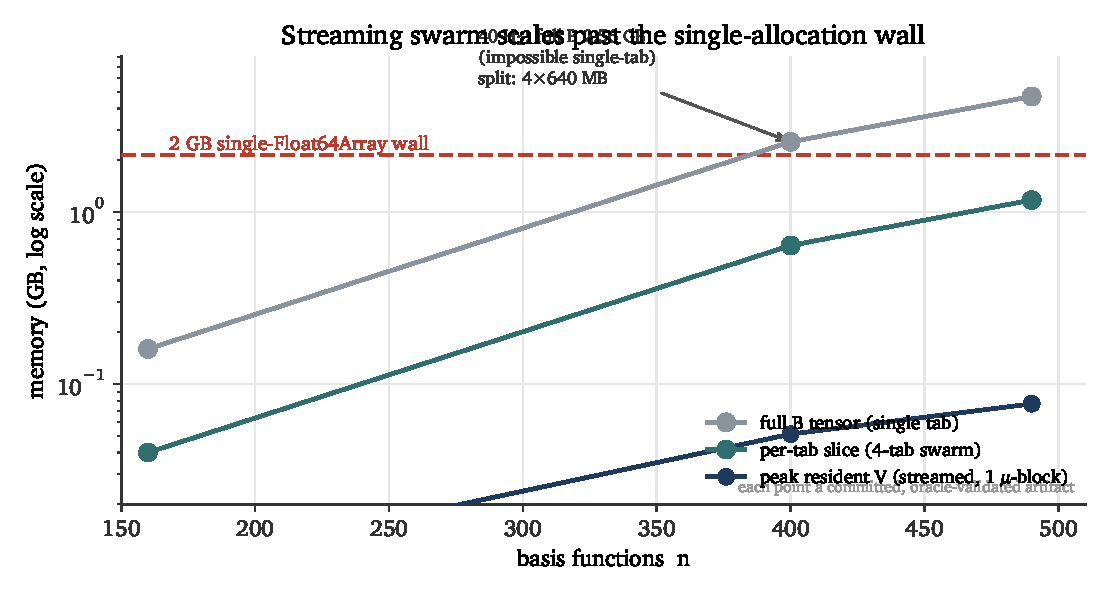
\includegraphics[width=0.92\textwidth]{fig-streaming-scale.pdf}
  \caption{Streaming swarm vs the 2\,GB single-allocation wall, H$_2$ lattice in
  cc-pVDZ. The full fitting tensor (grey) grows as $\sim n^2 n_{\mathrm{aux}}$
  and crosses the $2^{31}-1$ byte \texttt{Float64Array} ceiling (red) near
  $n\approx375$; beyond it the calculation is impossible on any single tab. The
  per-tab slice in a 4-tab swarm (teal) and the streamed peak resident $V$
  (navy, one $\mu$-block) both stay far below the wall, which is what lets the
  swarm run the $n{=}400$ ($2.56$\,GB) case. Each point is a committed,
  oracle-validated artifact.}
  \label{fig:streamscale}
\end{figure}

\section{Honest limitations}
\label{sec:limitations}

Per our research-grade discipline, failures are reported, not hidden:
\begin{itemize}
  \item \textbf{Multireference wall.} Linear acenes beyond pentacene develop
  open-shell-singlet/polyradical character; single-determinant RHF does not
  reliably converge for hexacene/heptacene (and convergence at octacene is
  luck, not signal). The swarm runs the full SCF to completion and returns
  finite energies, but RHF convergence there is method-limited --- UHF /
  spin-projected references are the fix.
  \item \textbf{Anthracene cc-pVDZ basin selection.} A delayed-DIIS recipe
  (damping 0.2, DIIS start at iter 8) avoids divergence but converges to a
  spurious lower-energy state; MOM / SAD-initial-guess is required for the
  physical ground state.
  \item \textbf{Density fitting gives no speedup yet} --- current CD-DF still
  builds the 4-index tensor before decomposing; aux-basis 3-index DF is the
  real win.
  \item \textbf{\Csixty{} runs only at STO-3G.} The streaming build removed the
  master's full-tensor peak, but \Csixty{} cc-pVDZ ($n\approx840$) has a fitting
  tensor of $\sim$26\,GB; even split across many tabs the \emph{sum} exceeds a
  16\,GB machine's RAM. Reaching it needs out-of-core slices or a larger host,
  not a software change.
  \item \textbf{SCF coordination is the wall above $n\approx400$.} At $M{=}49$
  H$_2$ ($n{=}490$) the \emph{build} scaled fine --- four tabs each built their
  1.18\,GB slice, a 4.7\,GB fit, with no full tensor anywhere --- but the
  per-iteration Fock gather stalled: broadcasting the density and gathering
  $(J,K)$ partials over \texttt{BroadcastChannel}'s structured clone (each
  $\sim$1.9\,MB at $n{=}490$), under multi-GB resident pressure, exceeded our
  per-iteration budget. The fix is \texttt{SharedArrayBuffer}-backed messaging
  for the per-iteration tensors (the build already streams); it is the next step
  for $n>400$, and is a transport limit, not a memory or correctness one.
\end{itemize}

\section{Related work}
\label{sec:related}

GPU-accelerated native quantum chemistry is mature: GPU4PySCF~\cite{gpu4pyscf},
QUICK~\cite{quick}, and VeloxChem~\cite{veloxchem} implement HF/DFT/Fock on
CUDA. None runs in a browser. Browser volunteer computing ---
Pando~\cite{pando}, Genet~\cite{genet}, QMachine~\cite{qmachine} ---
distributes generic workloads across tabs and devices but has not run
electronic structure. WebGPU is an actively characterized compute
target~\cite{webgpudispatch}. Web-based quantum-chemistry tools do exist ---
WebMO~\cite{webmo} and the Molecule Calculator~\cite{molcalc} --- but they are
server-client front-ends: the browser is a molecular editor and job monitor,
while the SCF runs on a native backend (GAMESS, Gaussian, etc.), and the
client-side methods are limited to RHF/STO-3G property estimation. webgpu-q
instead runs the entire HF/MP2/CCSD(T)/DFT/EOM stack \emph{in} the browser,
client-side, with no backend. On a literature search current to June~2026 we
find no published in-browser (client-side) electronic-structure implementation
at this method coverage, and none that distributes such a calculation across
browser tabs. Best-functional and benchmark context follows the GMTKN55
database~\cite{gmtkn55}; experimental reference data are from the NIST
CCCBDB~\cite{cccbdb}.

\section{Software availability and reproducibility}

\paragraph{Source.} The complete source is at
\texttt{github.com/abgnydn/webgpu-q}, public, MIT-licensed for original code;
portions ported from PySCF are Apache-2.0 with per-file attribution
consolidated in a root \texttt{NOTICE} (Apache-2.0 \S4(d)). The WebAssembly
integral kernels are Rust in \texttt{wasm-eri/}; the swarm in
\texttt{src/parallel/}; the chemistry in \texttt{src/chemistry/}.

\paragraph{Running it.} No installation, no account, no GPU driver: the
simulator runs in any WebGPU-capable Chromium with cross-origin isolation
(COOP/COEP) enabled. The swarm requires $N$ same-origin tabs; for the
cross-machine variant a PeerJS broker + STUN suffices. A reader can reproduce a
single-molecule HF run from a browser tab; the multi-tab swarm runs are
reproduced by opening $N$ tabs of the same origin.

\paragraph{Reproducibility harness.} Every experiment emits a JSON artifact
recording the git commit SHA, \texttt{navigator.userAgent},
\texttt{adapter.info} (vendor/architecture/device), WebGPU device limits, OS, a
UTC ISO-8601 timestamp, and the echoed \texttt{protocol}, \texttt{hypothesis},
\texttt{seed}, \texttt{warmup}, \texttt{trials}, and \texttt{pass\_bar}. No
\texttt{Math.random()} appears on any experiment path --- every random draw is
a named deterministic seed. Wall-clock is measured with
\texttt{performance.now()} bracketed by forced GPU sync (a mapped readback)
because \texttt{queue.submit} is non-blocking; 5 warmup samples are discarded
and 20 retained, reporting median/p10/p90/p99/std/IQR. Failing configurations
are committed with \texttt{status:"fail"} and a diagnosis rather than silently
rerun --- the honest-negative discipline that surfaced, for example, the acene
multireference wall and the anthracene cc-pVDZ basin-selection issue reported in
\S\ref{sec:limitations}. The committed \texttt{experiments/results/<date>/}
artifacts are the source of the level-1/2/3 and validation numbers; the swarm
scaling table (\S\ref{sec:scaling}) is produced by the end-to-end browser
benchmark specs under \texttt{e2e/}, each of which now emits the same
environment-stamped JSON artifact per run (git SHA, \texttt{adapter.info},
energy, $n$, $n_{\mathrm{aux}}$, iterations, and per-phase wall-time) under
\texttt{experiments/results/<date>/swarm/}.

\paragraph{Generative-AI disclosure.} Portions of the software, its
documentation, and this manuscript were drafted with the assistance of a large
language model used as a coding and writing aid. All AI-assisted output was
reviewed by the author; correctness of code was enforced by the test suite,
brute-force diagnostics, and PySCF cross-validation described in
\S\ref{sec:validation}, and every quantitative claim in this paper is traceable
to a committed experiment artifact rather than to model output.

\paragraph{Statements.} Sole author; no competing interests; no external
funding. Archived at Zenodo, concept DOI
\href{https://doi.org/10.5281/zenodo.20494382}{10.5281/zenodo.20494382}
(resolves to the latest version).

\section{Conclusion}

A full electronic-structure stack runs in a browser tab, validated against
PySCF, and a browser-tab swarm scales it to \Csixty{} without native code, a
data-center GPU, or an install. It does not aim to beat native suites on raw
speed --- on large correlated calculations it is far slower --- and its value
lies elsewhere: in removing the install, hardware, and cost barriers between a
learner and a real calculation, and in showing that the browser's memory
ceiling is not a hard limit but one that a tab swarm can raise. The entire
artifact is a URL, and a referee can re-run every number reported here.

\bibliographystyle{unsrt}
\bibliography{refs}

\end{document}
